% !TeX root = ../main.tex
\section{Исследование нелинейных свойств усилителя и измерение точки децибельной компрессии ($P_{1\text{dB}}$)}

\subsection{Теоретические сведения и методика проведения измерений}

При увеличении мощности входного сигнала амплитудная характеристика (АХ) реального усилителя перестает быть линейной вследствие физических ограничений активных полупроводниковых структур (насыщения по току коллектора/стока и ограничения динамического диапазона напряжением питания). 

Параметром, определяющим верхнюю границу линейного динамического диапазона усилителя, является \textbf{точка децибельной компрессии} ($P_{1\text{dB}}$). Она соответствует уровню мощности, при котором реальный коэффициент усиления каскада падает на 1~дБ по сравнению с коэффициентом усиления на начальном малосигнальном (линейном) участке характеристики:
\begin{equation}
OP_{1\text{dB}} = IP_{1\text{dB}} + K_1 - 1\text{ дБ},
\end{equation}
где $IP_{1\text{dB}}$ --- входная мощность компрессии в 1~дБ, $OP_{1\text{dB}}$ --- выходная мощность компрессии в 1~дБ, а $K_1$ --- малосигнальный коэффициент усиления.

\textbf{Порядок выполнения экспериментальных исследований (на частоте $f = 1\text{ ГГц}$):}
\begin{enumerate}
    \item \textbf{Калибровка потерь выходного тракта ($IL_2$):}
    \begin{itemize}
        \item собрана измерительная схема без исследуемого усилителя (рис.~24 методических указаний): Генератор ($+10\text{ дБм}$) $\to$ аттенюатор 20~дБ $\to$ Кабель 1 $\to$ адаптер $\text{SMA}(f)\text{--}\text{SMA}(f)$ $\to$ аттенюатор 10~дБ $\to$ Кабель 2 $\to$ Анализатор спектра; зафиксирован калибровочный уровень $P_1(1\text{ ГГц}) = -23.42\text{ дБм}$;
        \item из схемы исключены выходной аттенюатор 10~дБ и Кабель 2 (рис.~25 методических указаний; зафиксирован уровень $P_2(1\text{ ГГц}) = -12.40\text{ дБм}$;
        \item суммарные потери выходного измерительного плеча на частоте 1~ГГц составили:
        \begin{equation}
        IL_2 = P_2 - P_1 = -12.40 - (-23.42) = 11.02\text{ дБ}.
        \end{equation}
    \end{itemize}
    \item \textbf{Снятие амплитудной характеристики (рис.~26 методических указаний):} в измерительный тракт включен исследуемый усилитель с подачей напряжения питания. Мощность генератора сигналов варьировалась в диапазоне $P_{\text{вх}} \in [-10; +18]\text{ дБм}$ с шагом 2~дБ. На анализаторе спектра регистрировался уровень мощности $P_{\text{изм}}$.
    \item \textbf{Восстановление реальной мощности усилителя:} истинная выходная мощность $P_{\text{вых}}$ определялась компенсацией потерь выходного плеча:
    \begin{equation}
    P_{\text{вых}} = P_{\text{изм}} + IL_2 = P_{\text{изм}} + 11.02\text{ дБ}.
    \end{equation}
    \item \textbf{Определение точки компрессии:} строилась линейная асимптота по начальным точкам малого сигнала ($P_{\text{вх}} \in [-10; -6]\text{ дБм}$). Пороговое значение децибельного сжатия определялось из условия отклонения экспериментальной кривой от линейной аппроксимации ровно на 1~дБ ($\Delta = P_{\text{вых, идеал}} - P_{\text{вых}} = 1.0\text{ дБ}$).
\end{enumerate}

\subsection{Результаты экспериментальных исследований}

Результаты измерений амплитудной характеристики усилителя на частоте $f = 1\text{ ГГц}$ сведены в таблицу~\ref{tab:p1db}.

\begin{table}[H]
\centering
\caption{Экспериментальные данные и результаты расчета амплитудной характеристики ($f = 1\text{ ГГц}$)}
\label{tab:p1db}
\small
\begin{tabular}{|c|c|c|c|c|}
\hline
$P_{\text{вх}}$, дБм & $P_{\text{изм}}$, дБм & $P_{\text{вых}}$, дБм & $P_{\text{вых, идеал}}$, дБм & Сжатие $\Delta$, дБ \\
\hline
-10 & -18.39 & -7.37 & -7.33 & 0.04 \\
-8  & -16.49 & -5.47 & -5.55 & -0.08 \\
-6  & -14.83 & -3.81 & -3.77 & 0.04 \\
-4  & -13.20 & -2.18 & -1.99 & 0.19 \\
-2  & -12.02 & -1.00 & -0.21 & 0.79 \\
0   & -10.93 &  0.09 &  1.57 & 1.48 \\
2   & -10.05 &  0.97 &  3.35 & 2.38 \\
4   & -9.34  &  1.68 &  5.13 & 3.45 \\
6   & -8.64  &  2.38 &  6.91 & 4.53 \\
8   & -8.10  &  2.92 &  8.69 & 5.77 \\
10  & -7.66  &  3.36 & 10.47 & 7.11 \\
12  & -7.23  &  3.79 & 12.25 & 8.46 \\
14  & -6.86  &  4.16 & 14.03 & 9.87 \\
16  & -6.41  &  4.61 & 15.81 & 11.20 \\
18  & -6.07  &  4.95 & 17.59 & 12.64 \\
\hline
\end{tabular}
\end{table}

На основе полученных данных построен график амплитудной характеристики усилителя с выделением линейной асимптоты и точки $P_{1\text{dB}}$ (рис.~\ref{fig:p1db}).

\begin{figure}[H]
    \centering
    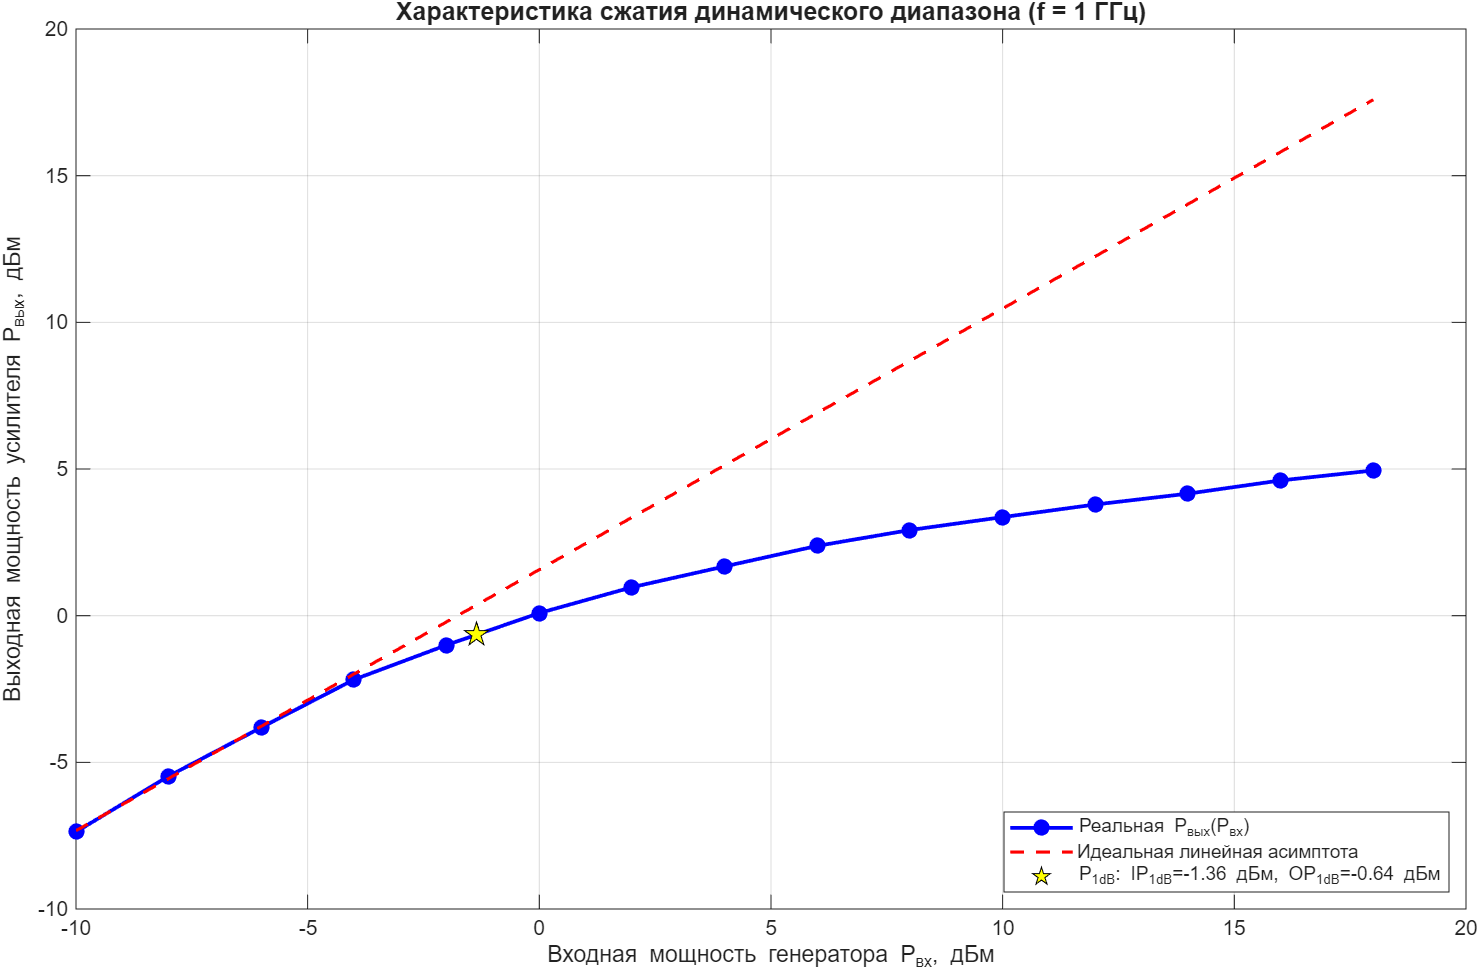
\includegraphics[width=0.88\textwidth]{Р1дб.png}
    \caption{Характеристика сжатия динамического диапазона и точка децибельной компрессии усилителя ($f = 1\text{ ГГц}$)}
    \label{fig:p1db}
\end{figure}

По результатам интерполяции экспериментальных данных точка децибельной компрессии составляет:
\begin{equation}
IP_{1\text{dB}} = -1.36\text{ дБм}, \qquad OP_{1\text{dB}} = -0.64\text{ дБм}.
\end{equation}

\subsection{Анализ результатов и выводы}

\begin{enumerate}
    \item \textbf{Линейный динамический диапазон:} В диапазоне входных мощностей от $-10\text{ дБм}$ до $-4\text{ дБм}$ характеристика усилителя близка к строго линейной с коэффициентом усиления каскада порядка $K_p \approx 11\text{ дБ}$ (с учетом предварительного ослабления входным аттенюатором). В этой области нелинейные искажения пренебрежимо малы.
    \item \textbf{Поведение в области компрессии и насыщения:} Начиная с уровня входной мощности $P_{\text{вх}} > -2\text{ дБм}$, наклон передаточной характеристики существенно уменьшается. Точка сжатия на 1~дБ достигается при входной мощности $IP_{1\text{dB}} = -1.36\text{ дБм}$ и выходной мощности $OP_{1\text{dB}} = -0.64\text{ дБм}$. При дальнейшем увеличении входной мощности до $+18\text{ дБм}$ усилитель переходит в режим глубокого насыщения с практически неизменной максимальной мощностью $P_{\text{sat}} \approx +5\text{ дБм}$.
    \item \textbf{Практическое значение точки $P_{1\text{dB}}$:} Значение $IP_{1\text{dB}} = -1.36\text{ дБм}$ задает строгую верхнюю границу линейного динамического диапазона усилительного каскада. Для сохранения целостности спектра широкополосных сигналов с переменной огибающей и предотвращения появления внеполосных продуктов интермодуляции рабочая точка усилителя должна выбираться на 10--12~дБ ниже точки $P_{1\text{dB}}$ ($P_{\text{вых.раб}} \le -11\text{--}-13\text{ дБм}$).
\end{enumerate}